\section{ROS framework}

\begin{frame}
\frametitle{ROS framework}
\begin{columns}
\column{0.3\textwidth}
Key components:
\begin{itemize}
\item Nodes
\item Topics \& Messages
\item Parameters
\item Launch files
\item Packages
\item ROS filesystem, network, tools \& community
\item ...
\end{itemize}
\column{0.7\textwidth}
\begin{center}
\begin{figure}[!htb]
\centering
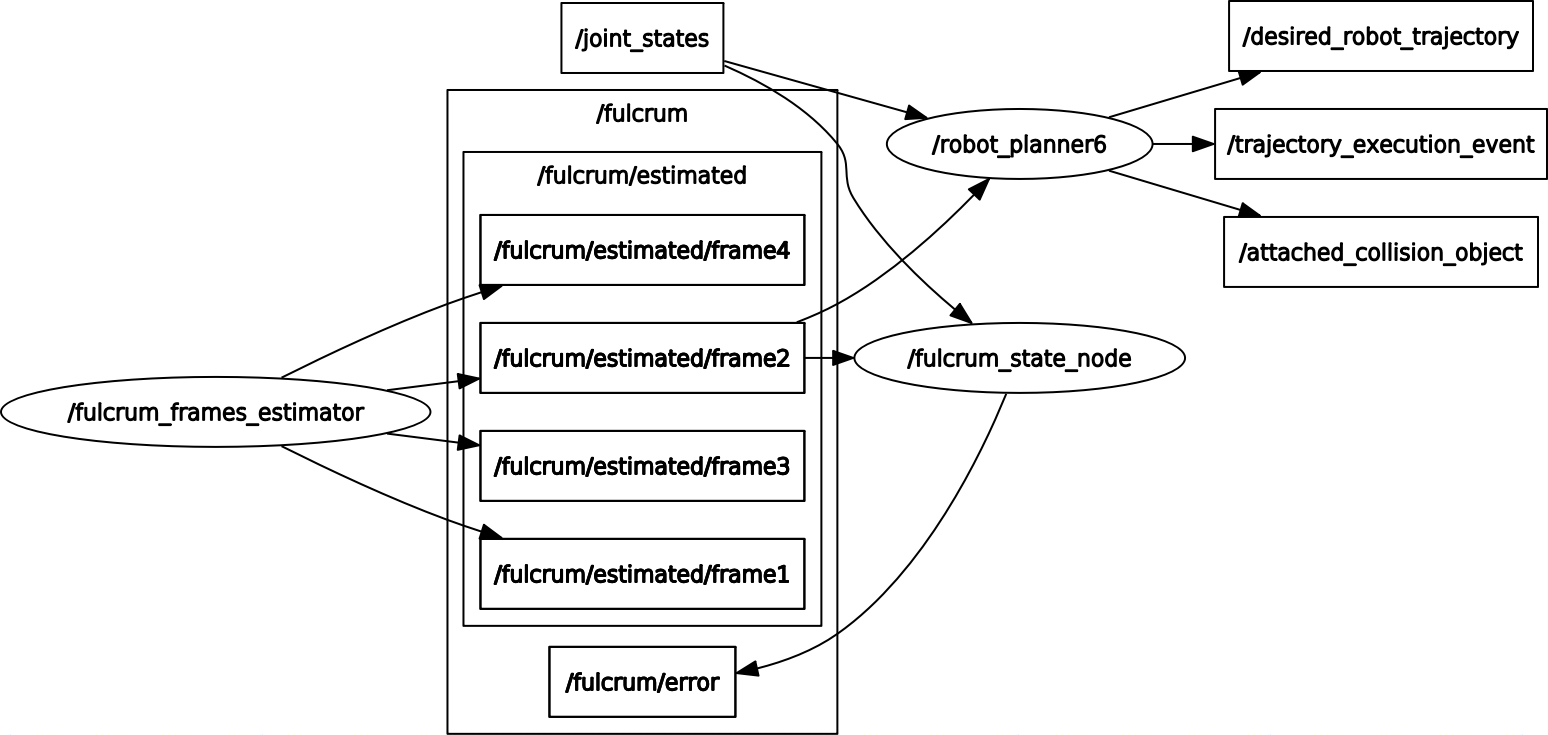
\includegraphics[width=\textwidth]{../images/robot_planner6/topics-and-nodes.png}
\caption{Subset of ROS nodes and topics used for the robot-planner6 experiment}
\end{figure}
\end{center}
\end{columns}
\end{frame}

\begin{frame}
\frametitle{Gazebo simulation environment}
\end{frame}

\begin{frame}
\frametitle{Visualization with RViz}
\end{frame}

\begin{frame}
\frametitle{Motion Planning with Moveit}
Moveit motion planning parameter values outside and inside of surgical site:
\begin{itemize}
	\item \textbf{Position tolerance}: 50 - 500μm, 5μm
	\item \textbf{Orientation tolerance}: 0.00005deg, 0.000005deg
	\item \textbf{Maximum planning time}: 5-10s, 5s
	\item \textbf{Replanning allowed}: true
	\item End-effector \textbf{interpolation step}: 1mm
	\item \textbf{Base frame}: world (universal)
	\item \textbf{Jump threshold}
	\item \textbf{Planner algorithm}: RRTConnect
	\item \textbf{Maximum planning attempts}: 6
	\item \textbf{Fraction}
\end{itemize}
\end{frame}

\begin{frame}
\frametitle{Tools, Packages and Libraries}
\begin{columns}[t]
\column{0.5\textwidth}
\begin{itemize}
\item \textbf{tf2}: keep track of multiple coordinate frames, apply transformations
\item \textbf{geometry\_msgs}
\item \textbf{Eigen}: linear algebra
\item \textbf{OpenCV2}: computer vision
\item \textbf{numpy}
\item \textbf{actionlib}
\item State machines with \textbf{Smach}
\end{itemize}

\column{0.5\textwidth}
\begin{itemize}
\item  ros-industrial/\textbf{kuka\_experimental }
\item \textbf{barrett\_hand}
\item \textbf{gazebo-pkgs}
\item \textbf{moveit-pkgs}
\item ...
\end{itemize}
\end{columns}
\end{frame}